\newpage
\section{Постановка задачи оптимизации}
Даны конечный неориентиованный граф \(G=(V,E)\), весовая функция \(w:E\rightarrow \mathbb{N}\) и подмножество \(S = \{s_1, s_2,...,s_k\}\subset V\). Требуется найти подмножество \(T\subset E\) наименьшего веса, чтобы в графе \(G - T\) все вершины множества \(S\) лежали в разных компонентах связности.

\section{Формулировка задачи распознавания, доказательство \(NP\)-полноты}
\subsection{Формулировка задачи распознавания}
Даны конечный неориентиованный граф \(G=(V,E)\), весовая функция \(w:E\rightarrow \mathbb{N}\), подмножество \(S = \{s_1, s_2,...,s_k\}\subset V\) и вес W. Требуется определить: существует ли подмножество \(T\subset E\) такое что в графе \(G - T\) все вершины множества \(S\) лежали в разных компонентах связности и \(w(T) \leq W\).

\subsection{Доказательство \(NP\)-полноты}
\begin{theorem}
Задача распознавания является NP-полной, если граф планарен, веса ребер
ограничены и максимальная степень вершины равна 3.
\end{theorem}
\textbf{Доказательство}
\\Задача распознавания для Minimum Multiway Cut находится в NP (сертификат можно проверить за полиномиальное время с помощью поиска в глубину). Для завершения доказательства необходимо показать полиномиальное преобразование из некоторой известной NP-полной задачи. В данном доказательстве это будет задача 3-SAT.
В задаче о 3-SAT даны множества \(X=\{x_1, x_2,...,x_n\}\) переменных и \(C=\{c_1, c_2,...,c_n\}\) 3-элементных формул, т. е. подмножеств множества литералов из \(X\), где если \(x_i\) является переменной, то соответствующие ей литералы \(x_i\) и \(\overline{x_i}\). Требуется определить: 
существует ли множество \(T \in X\), так что \(T\) содержит ровно одно из \(x_i\) и \(\overline{x_i}\) и \(c_i=true\) \(\forall{i\in (1, n)}\)  
Двудольный граф \(G_{X,C}\), связанный с этой задачей, имеет \(X\cup C\) в качестве множества вершин и ребро между вершинами \(x_i\) и \(c_j\), если \(c_j\) содержит любой из литералов \(x_i\) или \(\overline{x_i}\).
\\
\\Для преобразования к планарной задаче Multiway Cut  будем использовать ограниченный
вариант PLANAR 3-SAT, в котором допускаются формулы размера два и три, но
требуется, чтобы каждый литерал имел ровно третью степень в \(G_{X,C}\), причем один из ее литералов встречался в двух формулах, а другой в одной. Можно доказать NP-полноту преобразованием локальной замены из 3-SAT. Пусть \(X,C\) обозначает экземпляр задачи 3-SAT, как указано выше. Не умоляя общности, будем считать \(x_i\), и \(\overline{x_i}\) содержатся в \(\bigcup_{j=1}^{m}c_j\) для всех \(x_i\): если \(\overline{x_i}\) не встречается ни в одной формуле также можно считать, что \(x_i=true\), и, следовательно,
все формулы, содержащие \(x_i\), всегда выполняются. Теперь можно убрать эти формулы из выражения. Таким образом, каждый
литерал встречается как минимум в двух формулах, и все литеральные вершины в \(G_{X,C}\) имеют степень не менее двух.

\\
\\Метод преобразования такого графа \(X, C\) в граф \(X^'\), \(C^'\) нашего варианта 3-SAT включает замену старых литералов, добавление некоторых новых формул и изменение старых формул. Во-первых, заменим каждую переменную \(x_i\) набором \(degree(xi)\) новые переменные:
\(x_{i,1}, x_{i,2}, . . . , x_{i,degree(x_i)}\). Вместе они образуют цикл длины \(2degree(x_i)\) в \(G_{X^{'},C^'}\), как показано на рис. 1 для случая, когда \(degree(x_i) = 5\).
Добавленные формулы гарантируют, что все новые литералы должны иметь одно и то же значение истинности во всех формулах. Построение X',C' завершается модификацией старых дизъюнктов таким образом, чтобы новая
модель, соответствовала новому графу. Для каждого вхождения литерала \(x_i\) в формулу \(c_j\), должно быть ребро в \(G_{X^{'},C^{'}}\) между \(c_j\) и новой переменной \(x_{i,k}\). Заменяем литерал \(x_i\)
новым литералом \(x_{i,k}\). Несложно проверить, что новая модель имеет нужный формат
и является выполнимой тогда и только тогда, когда была выполнима исходная модель.
\begin{figure}[hbt!]
\centering
    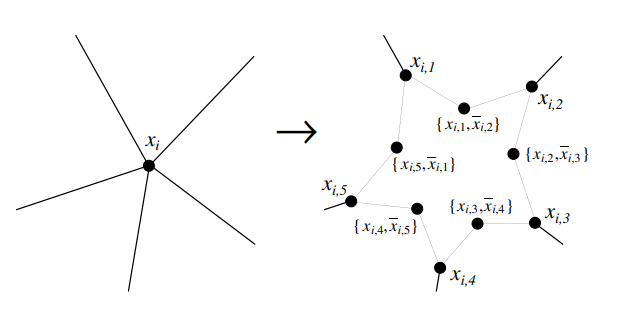
\includegraphics{Conversion3SAT}
    \caption{3-SAT преобразование.}
\end{figure}
\\
\\Чтобы завершить доказательство теоремы, покажем теперь, как преобразовать экземпляр \({X,C}\)
из 3-SAT к экземпляру планарного Multiway Cut, в котором все
веса равны пяти или меньше, и все вершины имеют степень три или меньше. Для этого используем подход "component design", описанный в [6]. На рис. 2 показаны компоненты, которые мы будем использовать для представления литералов и
формул.
\begin{figure}[hbt!]
\centering
    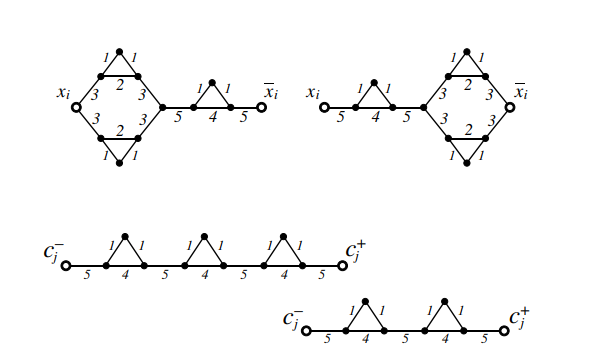
\includegraphics{Conversion3SAT2}
    \caption{Преобразование литералов и формул.}
\end{figure}
\\Литерал \(x_i\) представлен одной из двух структур в верхней части рисунка. В первой, если литерал \(x_i\) встречается в двух формулах, во второй - если  \(\overline{x_i}\) встречается в двух формулах. Терминалы в этих структурах — это вершины, помеченные \(x_i\) и \(\overline{x_i}\). Соединительные треугольники этих структур представляют собой три треугольника, веса ребер которых равны 1,1,2 или 1,1,4.
Основания соединителя — это ребра веса 2 и веса 4 в этих треугольниках, ребра соединителя
являются ребрами веса 1, а вершины соединителей являются вершинами степени 2 треугольников. Каждый соединительный треугольник, основание, ребро и вершина будут рассматриваться как литерал, помеченный ближайшим к нему терминалом.
\\Формула \(c_j\) представлена одной из двух формул в нижней части рисунка, первая, если
\(|c_j| = 3\), второе, если \(|c_j| = 2\). Здесь терминалами являются вершины с номерами \(c_j^-\)
и \(c_j^+\). Соединительные треугольники — это треугольники, веса ребер которых равны 1, 1, 4, а основания соединителей, ребра соединителей и вершины соединителей снова являются ребрами веса 4, ребрами веса 1 и вершинами степени 2 этих треугольников. Получается, что треугольников-соединителей ровно столько, сколько литералов в выражении. Предположим, что каждому соединителю назначено представление отдельного литерала.
Важно, что все структуры на рис. 2 имеют максимальную степень три. Чтобы завершить построение графа Multiway Cut G[X,C], нужно только соединить формулы и литералы. Это делается путем добавления ребер веса 2, как показано на рис. 3. Получим нужное количество соединительных вершин (по определению ограниченного 3-SAT), чтобы соединить один к одному со всеми соединителями, инцидентными ровно одному ребру веса 2. Из этого следует, что максимальная степень полученного графа G[X,C] равна трем. Граф G[X,C] будет планарным, так как \(G_{X,C}\) планарный.
\begin{figure}[hbt!]
\centering
    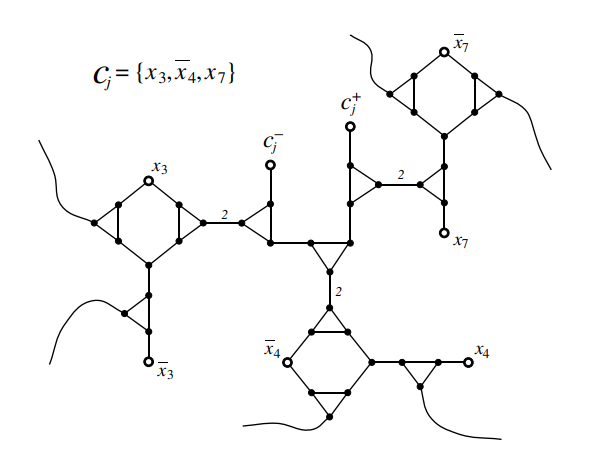
\includegraphics{Conversion3SAT3}
    \caption{Соединение компонент в доказательстве теоремы 1.}
\end{figure}
\\Единственное, что осталось показать, — это верхнюю границу B искомого разреза. Покажем, что B = 10n + 4m, где n и m — количество литералов и формул в ограниченном 3-SAT. Описанная конструкция строится за полиномиальное время. Чтобы завершить доказательство того, что это полиномиальное преобразование, нужно показать, что следующие два утверждения эквивалентны:
\\(1) Экземпляр PLANAR 3-SAT X,C имеет решение.
\\(2) Существует множество \(E^'\) ребер в \(G[X,C]\), общий вес которых не превышает B и удаление которых
уберет все пути между 2n + 2m терминалами.
Предположим, что множество T существует. Тогда разрез можно построить. Для каждой формулы \(c_j\) выбираем литерал в \(c_j \cap T\) (как минимум один должен существовать, так как T - решение задачи 3-SAT) и удалить все ребра соответствующего соединительного треугольника из \(c_j\) в \(G[X,C]\). Для каждой переменной надо удалить все три ребра из каждого соединительного треугольника, представляющего литерал не в \(T\). В конце надо удалить каждое связующее ребро, которое не является смежным с уже удаленным соединительным треугольником. Пусть \(E^'\) будет набором удаленных ребер.
\\Во-первых, отметим, что \(E^'\) обладает требуемыми свойствами разреза. Получается, что по крайней мере один конец каждого оставшегося ребра должен иметь степень 1 после удаления \(E^'\). Таким образом, ни один путь между терминалами не может проходить через ребро. Следовательно, если существует какой-либо путь, соединяющий терминалы, он должен либо связывать пару терминалов того же литерала или пара \(c_j\) находится в той же формуле. В первом случае все такие пути должны проходить через соединительные треугольники, представляющие оба литерала, и поэтому должны быть разорваные, так как мы удалили все соединительные треугольники, представляющие один из литералов. В другом случае, любой такой путь должен проходить через все соединительные треугольники \(c_j\), и поэтому будет разорван.
Теперь \(w(E^') = 10n + 4m = B\), поэтому \(E^'\) удовлетворяет ограничению и является желаемым разрезом. Чтобы убедиться в этом, разделим ребра G[X,C] по-другому. Сгруппируем каждое связующее ребро веса 2 с четырьмя ребрами веса 1 из соединительных треугольников, которым он инцидентен, и назовем группу из 5 ребер структурой соединения. См. рис. 4, где ребра \({a,c}, {b,c}, {c,d}, {d,e} и {d, f}\) составляют структуру соединения, соединяющая структуры для формулы \(c_j\) и литерала \(x_i\). 
\begin{figure}[hbt!]
\centering
    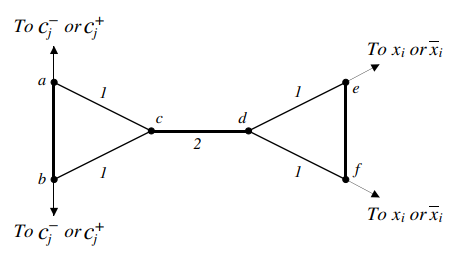
\includegraphics{Conversion3SAT4}
    \caption{Пример связи между формулой и литеральным компонентом.}
\end{figure}
Покажем, что для любой структуры общий вес удаленных ребер равен ровно 2. Связующее ребро с весом 2 удаляется тогда и только тогда, когда ни одно из ребер с весом 1 не было удалено. Предположим, что одна из пар ребер веса 1 была удалена. Если это пара из треугольника формулы, то соответствующий литерал должен быть истинным. Если это из треугольника литерала, это означает, что соответствующий литерал должен быть ложным. Поскольку оба утверждения не могут выполняться одновременно, только два ребра веса 1 могут находиться в \(E^'\). Таким образом, общий вес ребер, удаленных из структуры, равен двум, а общий общий вес ребер удаленных из структур вдвое больше, чем таких структур, то есть \(6n\). Теперь рассмотрим структуры формул и литералов. Мы удалили по одному ребру веса 4, общим весом \(4m\). Из последнего мы удалили либо одно ребро веса 4 или два веса 2, и общей вес \(4n\). Это предельный результат из которого следует, что
\(w(E^{'}) = 6n + 4m + 4n = B\), что и требовалось.
И наоборот, предположим, что существует множество \(E^'\) с указанными свойствами. Покажем, что X,C
имеет решение. Начнем с последовательности лемм о «нормальной форме».Предположим, что \(E^'\) является множеством минимального веса, удовлетворяющим указанным свойствам.
\begin{lemma} Предположим, что \(e\) — ребро, инцидентное вершине \(v\) степени 3. Если вес \(e\) больше или равен сумме весов двух других ребер, инцидентных \(v\), то \(e\) не лежит в \(E^'\).
\end{lemma}
\textbf{Доказательство} Предположим, что \(e \in E^'\), и рассмотрим результат удаления \(e\) из \(E^'\) и замены его всеми другими ребрами, инцидентными \(v\) и еще не принадлежащие \(E^'\). Это не увеличит вес \(E^'\). Это также не может создать путь между терминалами в остаточном графе. Если это так,
этот путь содержит \(e\). Поскольку \(v\) теперь имеет степень один в остаточном графе, то \(v\) - один из концов пути, а значит терминал. Это невозможно, так как в модели нет вершины степени 3, являющейся терминалом (рис. 1 и 2).
Как следствие леммы 1, в дальнейшем будем предполагать, что ни один из весов
ребра в любой структуре формулы не находятся в \(E^'\), и ни одно из ребер веса 3 или 5 не находится в  структуре литерала.
\begin{lemma} Если какое-либо ребро в цикле G[X,C] лежит в \(E^'\), то таких ребер по крайней мере два.
\end{lemma}
\textbf{Доказательство} Если \(e\) — единственное ребро из данного цикла в \(E^'\), то удаление \(e\) из \(E^'\) уменьшит \(w(E^')\) без добавления новых связей, что противоречит нашему предположению о том, что \(E^'\) было минимальным разрезом.
\begin{lemma} Не более одного основания соединителя (ребро веса \(4\)) в любой структуре формулы находится в \(E^'\).
\end{lemma}
\textbf{Доказательство} Предположим, что структура для \(c_j\) имеет два ребра веса \(4\) в \(E^'\). Рассмотрим общую структуру формулы, включая все соединительные ребра, как на рис. 2. По лемме 2 можно считать, что \(E^'\) содержит по крайней мере одно ребро соединителя, примыкающее к каждому содержащемуся в нем основанию соединителя, и, следовательно, суммарный вес ребер из структуры формулы, находящихся в \(E^'\), не меньше 10. Рассмотрим следующую модификацию \(E^'\): удалим одно из двух оснований разъема и добавьте все оставшиеся ребра разъема (их может быть не более четырех). Эта модификация не увеличивает вес \(E^'\). Он также не может создать никаких новых межтерминальных путей в остаточном графе: поскольку все коннекторы ребра теперь удалены, такой созданный путь мог связать только \(c_j^-\) и \(c_j^+\), но эти терминалы остаются разделены, так как одно из ребер веса 4 остается в \(E^'\).
\begin{lemma} Для каждой переменной \(x_i,E^'\) либо содержит базу соединителя, представляющую литерал \(x_i\) или базу, представляющию литерал \(\overline{x_i}\), но не оба.
\end{lemma}
\textbf{Доказательство} Давайте рассмотрим всю структуру литерала, включая все ребра соединителя, как показано на рис. 2. По лемме 1 в \(E^'\) нет ни одного ребра веса 3 и веса 5, значит мы должны либо удалить основание веса 4 или оба основания веса 2, если мы хотим отключить терминал \(x_i\) от терминала \(\overline{x_i}\). Из леммы 2, если мы удалим одно из оснований веса 2, мы должны удалить оба. Так что нужно исключить ситуацию, в которой мы удаляем все три базовых соединителя. Также необходимо удалить по крайней мере по одному ребру соединителя из каждого треугольника соединителя по лемме 2. Таким образом, общий вес ребер из структуры, которая находилась бы в \(E^'\), был бы минимум 11. Рассмотрим следующую модификацию \(E^'\): удалить два основания веса 2 и добавить все оставшиеся ребра соединителей (их может быть не более трех). Эта модификация не может создать новые пути в остаточном графе, поскольку \(x_i\) остается отделенным от \(\overline{x_i}\) и нет пути, включающего терминал, кроме двух. Кроме того, снижается вес \(E^'\). Опять пришли к противоречию минимальности \(E^'\).
\begin{lemma} Для каждой структуры связи \(E^'\) содержит только ребра веса два.
\end{lemma}
\textbf{Доказательство} Сначала покажем, что сумма должна быть не менее двух. Это будет означать, что их ровно два, так как по леммам 3 и 4 \(E^'\) содержит соединительные базы суммарного веса не менее 4m + 4n. Получается вес для ребер структур соединителей не более \(6n\), а таких структур \(3n\). Согласно леммам 1, 3 и 4, вершины \(a\) и \(b\) остаются соединенными с конечными пунктами в остаточном графе, а вершины e и
f остаются подключенными к терминалам. Но это значит, что в остатке будет путь от терминала литерала к терминалу формулы, если мы не удалим связующее ребро веса 2 или два ребра веса 1 из одного соединительного треугольника. В любом случае вес двух удаленных ребер не менее двух.
\\\\Теперь мы можем доказать наше утверждение о том, что решение T должно существовать. Для каждой переменной \(x_i\), поместите литерал, основание которого не находится в \(E^'\), в T. По лемме 4 это удовлетворяет всем формулам. Рассмотрим пункт \(c_j\), и пусть z будет литерал, соответствующий сломанной базе соединителя. По лемме 3 существует единственный такой z. Теперь рассмотрим структуру ссылки, соединяющей структуру для \(c_j\) и структуру литерала для z. Важно, что при нашем выборе z ребро (a,b) находится в \(E^'\). Если бы z не было в T, то ребро (e, f) также было бы в \(E^'\). Таким образом, по лемме 2 хотя бы одно соединительное ребро из каждого соединительного треугольника должно лежать в \(E^'\).
Заметим, что если в \(E^'\) нет других ребер из структуры соеденителей, все равно будет путь из одного из ребер a, b к одному из e, f внутри структуры. По леммам 1, 3 и 4 это означало бы, что существует
путь от терминала литерала к терминалу формулы - противоречие. Таким образом, T - искомое решение, и мы действительно построили полиномиальное преобразование, то есть и теорема 1 верна.
\begin{theorem} Задача Minimum Multiway Cut является NP-полной для планарных графов если веса всех ребер равны и степени вершин ограничены.
\end{theorem}
\textbf{Доказательство} Это прямое следствие предыдущего доказательства. Наша конструкция все еще работает, если заменить каждое ребро веса w на w параллельных путей, каждый из которых состоит из двух ребер веса 1. Поскольку ни одна вершина в нашей конструкции не имела инцидентных рёбер с суммарным весом больше 11, получится граф с максимальной степенью 11, и все ребра с весом 1. 
\section{Исследование частных случаев}
\subsection{Min-Cut (\(k = 2\))}
Даны конечный неориентиованный граф \(G=(V,E)\), весовая функция \(w:E\rightarrow \mathbb{N}\) и вершины \(U\) и \(V\). Требуется найти подмножество \(T\subset E\) наименьшего веса, чтобы в графе \(G - T\) вершины \(U\) и \(V\) лежали в разных компонентах связности.
\\\begin{definition}
Поток - это действительная функция \(x:V\times V \rightarrow R\), удоволетворяющая условиям:
\\1) \(x(u,v)= -x(v,u)\) (антисимметричность);
\\2) \(x(u,v)\leq c(u,v)\) (ограничение пропускной способности), если ребра нет, то \(x(u,v)=0\);
\\3) \(\sum_v x(u,v)=0\) для всех вершин u, кроме U и V (закон сохранения потока).
Величина потока x определяется как \(|x|=\sum_v x(U,v)\)
\end{definition}

Был предложен следующий алгоритм для нахождения min-cut [1]:
\\\\Алгоритм нахождения максимального потока
\\\textbf{Шаг 0} Пусть \(x = (x_{ij})\) — любой допустимый путь из U в V. Дать узлу U постоянную метку \((-, \infty)\).
\\\\\textbf{Шаг 1} (Маркировка и сканирование)
\\(1.1) Если все помеченные узлы были отсканированы, перейти к шагу 3.
\\(1.2) Найти помеченный, но не просканированный узел \(i\) и просканировать его следующим образом:
каждой дуге \((i, j)\), если \(x_{ij} < w_{ij}\) и \(j\) не помечен, присвоить \(j\) метку \((i^+, \delta_j)\), где
\begin{center}
{\(\delta_j = min\{w_{ij}-x_{ij}, \delta_j\}.\)}
\end{center}
Для каждой дуги \((j, i)\), если \(x_{ij} > 0\) и j не имеет метки, присвоить \(j\) метку \((i^-, \delta_j)\),
где
\begin{center}
{\(\delta_j = min\{x_{ji}, \delta_j\}.\)}
\end{center}
\\(1.3) Если узел t помечен, перейти к шагу 2; в противном случае перейти к шагу 1.1.
\\\\\textbf{Шаг 2} (Приращение) Начиная с узла t, использовать индексные метки для построения
увеличивающего пути. (Метка на узле \(I\) указывает на последний узел
в пути, метка на этом узле указывает на предпоследний узел и так
далее.) Увеличить поток, увеличив и уменьшив дуговые потоки на \(\delta_I\), как
обозначаются надстрочными индексами на метках указателя. Стерреть все метки, кроме
метка на узле s. Перейти к шагу 1.
\\\\\textbf{Шаг 3} (Построение минимального разреза) Существующий поток максимален. A
разрез минимальной мощности получается размещением всех помеченных узлов в \(S\)
и все непомеченные узлы в \(T\).

\\\\Оценить сложность вычислений можно следующим образом. Пусть
\(m\) — количество дуг. Не более \(2m\) сканирований дуг, за которыми следуют возможные
маркировки узлов, которые нужны когда строится увеличивающий путь.
Требуется не более \(\nu\) дополнений, где
\(\nu\) – максимальное значение потока. Таким образом, сложность алгоритма составляет \(O(m\nu\)) - полиномиальная.

\section{Точный экспоненциальный алгоритм решения оптимизационной задачи с оценкой его сложности}

Можно построить точный экспоненциальный алгоритм решения задачи поиска минимального разреза. Решение основывается на полном переборе возможных множеств ребёр. 
\\\\\textbf{Шаг 0:}
\begin{itemize}
    \itemВведём переменную минимального суммарного веса всех удаленных ребер в рассматриваемом решении
    \itemВведём битовую строку с длиной равной количеству ребер в графе и будем увеличивать ее на один после каждого шага цикла
\end{itemize}
\\\textbf{Шаг 1:}
\begin{itemize}
    \itemРассмотрим конкретную битовую строку, которая представляет из себя набор ребер
    \itemПроверим, является ли он разрезом для \(k\) терминалов
\end{itemize}
\\\textbf{Шаг 1.1:}
\begin{itemize}
    \itemБудем запускать поиск в глубину из каждого терминала 
    \itemЕсли в ходе работы поиска в глубину мы дошли до другого терминала, значит данный набор ребер не является разрезом для \(k\) терминалов. Переходим к следующему набору ребер
\end{itemize}
\\\textbf{Шаг 2:}
\begin{itemize}    
    \itemСчитаем сумму ребер данного разреза и обновляем переменную минимума
    \itemСохраняем набор ребер разреза как минимальный
    \itemПереходим к следующему набору ребер
\end{itemize}
\\
\vspace{5mm}
\\\textbf{Оценка сложности:}
Количество рассматриваемых наборов ребер \(2^m\), где m - количество ребер. При этом \(n-1\leq m\leq{n^2}\). Проверка каждого набора ребер (поиск в глубину) занимает \(O(n+m)\).Тогда общая сложность алгоритма в худшем случае \(O(2^{n^2}(n + m))\).
\section{Полиномиальный приближенный алгоритм решения оптимизационной задачи}

Можно построить приближенный алгоритм решающий задачу Minimum Multiway Cut за полиномиальное время, используя изолирующие разрезы минимального веса. Изолирующий разрез для терминала \(s_i\) это набор ребер, который отделяет \(s_i\) от других терминалов в \(S\).

\\\\Нахождение изолирующего разреза минимального веса[3,5] для теминала \(s_i\) сводится к нахождению минимального разреза (Min-Cut). Преобразуем данный граф в новый, в котором суперузел \(s^{'}_i\) заменяет остальные
терминалы \(S-\{s_i\}\), где ребра, выходящие из \(s^{'}_i\)
соответствуют ребрам, выходящим из любого из терминалов в \(S-\{s_i\}\). Теперь найдем минимальный разрез между \(s_i\) и \(s^{'}_i\)
в этом новом графе, который представляет собой минимальный изолирующий разрез для \(s_i\)
в \(G\).

\\\\В нашем алгоритме мы сначала вычислим изолирующий разрез минимального веса \(C_i\) для каждого терминала \(s_i\). Объединение любых \(k-1\) из этих \(k\) изолирующих разрезов будет решением для исходного графа, потому что такой разрез изолирует каждого из первых \(k-1\) терминалов
и, таким образом, он также изолирует последний терминал. Покажем, что отношение общего веса
\(k-1\) легчайших изолирующих разрезов к весу оптимального разреза не превышает \((2-\frac{2}{k})\). 
\begin{theorem}
Суммарный вес \(k-1\) легчайших изолирующих разрезов для множества терминалов \(S\)
не более чем в \((2-\frac{2}{k})\) раза превышает вес оптимального разреза.
\end{theorem}
\textbf{Доказательство}
\\Пусть \(T\) — оптимальный разрез для \(S\). Если удалить множество ребер \(T\) из
\(G\), должно остаться k компонент связности \(V_1, V_2, . . . , V_k\), где \(V_i\) содержит \(s_i\) в качестве терминала. Пусть \(T_i\) — множество ребер в \(G\) между \(V_i\) и \(V-V_i\) и \(T_i\) представляет изолирующий разрез для \(s_i\).
\\\\Заметим, что каждое ребро \(e\in T\) должно проходить между двумя компонентами, назовем их \(V_i\) и \(V_j\), так что \(e\in T_i\) и \(e\in T_j\). Таким образом, каждый член из суммы весов в \(w(T)\) появляется дважды в сумме весов в \(w(T_1) + w(T_2) + . . . + w(T_k)\). Следовательно:

\[\sum_{i=1}^{k}w(T_i) = 2w(T) \tag{1}\] 
Не умоляя общности предполагаем, что разрез \(T_k\) имеет максимальный вес среди всех разрезов \(T_i\). Можно утверждать, что:
\[\sum_{i=1}^{k-1}w(T_i) \leq{2(\frac{k-1}{k})w(T)} = (2-\frac{2}{k})w(T) \tag{2}\] 
Теперь вспомним, что каждый \(T_i\) является изолирующим разрезом для одного из терминалов \(s_i\). 
Однако, поскольку мы нашли изолирующие разрезы минимального веса для каждого терминала, мы обязательно имеем \(w(Ci) \leq{w(Ti)}\) для каждого \(i\). Используя уравнение (1) получаем:
\[\sum_{i=1}^{k-1}w(C_i)\leq{\sum_{i=1}^{k-1}w(T_i) \leq{2(\frac{k-1}{k})w(T)}} = (2-\frac{2}{k})w(T) \tag{3}\] 
Заметим, что \(\sum_{i=1}^{k-1}w(C_i)\) не меньше суммы \(k-1\) легчайших изолирующих разрезов, что завершает доказательство.
\\\\Сложность приведенного алгоритма \(O(knmlog(n^2/m))\) [3]